\chapitre{L’âge du Nutrisuz}{Assis dans son officine } {en train de jouer à la dame de pique sur son terminal de quanticordi et de se récurer les ongles, Timothée qui ne pense déjà plus aux sacs de madame Loubert, réfléchit sur sa vie de grand timide qui n’arrive jamais à sourire en public et de pestiféré qui craint ses collègues de travail, ces imbéciles qui le traitent de «Motté» et parfois de «p’tit gros qui saute la grande folle du manger mou». Effectivement, son ami, Shimoune Saint-Pierre, est gai comme phoque et ne se gêne pas pour assumer, particulièrement au Centre nutritionnel où il travaille, son exubérante homosexualité, au demeurant inoffensive.}

Tous deux se sont connus aux réunions du Comité de déontologie de l’établissement où Timothée siège en tant que représentant des cadres de premier niveau, les CS-1, et Shimoune en tant que délégué du personnel de soutien. Comme ils ont tous deux été désignés unilatéralement par la direction générale, qu’ils n’ont absolument pas l’appui de leurs pairs et qu’ils sont les deux seuls participants – un bien grand mot - à trouver les séances surréalistes, ils ont rapidement fraternisé.

Un cyberpsy, personnage de synthèse parfois plus humain que les vrais psychologues, a naguère révélé à Timothée qu’il devait son trouble de personnalité à sa mère, en fait, à la tyrannie de sa mère, la redoutable Maririou. Une Rioux avec un X, une Rioux musicalement virtuose, un air bête qu’on a envie de fesser, une fendante qu’on aime haïr, une grosse tête omnisciente, une force sinueuse, une manipulatrice experte, une inquisitrice qui ferait peur aux Dominicains de l’Opus Dei, une vaginocrate qui n’a, de sa vie, jamais perdu le nord, une écorchée vive qui, au cours des 43 dernières années, a été cruellement privée de fibre maternelle.

Mais attention, c’est quand même lui, Romain, qui a eu l’idée de cet invraisemblable prénom de Timothée-Milet, davantage l’expression d’un antagonisme handicapant ou d’un particularisme peu accommodable, que d’un prénom. Lui, le nono prostré dont on fait les gorges chaudes, il porte le nom d’un fonceur, d’un poète, d’un musicien, d’un réformateur, d’un maître à penser ayant fait école. Timothée de Milet ! Si Dieu existait vraiment, jamais il n’aurait permis tel déprédation d’un grand nom, telle offrande à la méchanceté des hommes de 2033 ! Lui, Timothée, fils de Marie Rioux et Romain Tardif, il n’est musicien que parce qu’on le lui a imposé. S’il est devenu joueur de trombone, un instrument qu’il a appris à haïr, c’est avec une fourche à foin lui piquant le bas du dos.

Il se considère comme un «dommage collatéral» ayant dû apprendre à vivoter sans blonde, cela grâce aux psychosévices de cette terrible femme, ainsi qu’ à la nature de l’air qu’elle a pompé dans sa vie d’éternel perdant et dans celle de Romain, son compagnon des 53 dernières années. En fait, Timothée n’en a jamais eu de blonde, pas plus qu’il n’envisage en avoir. Pas qu’il n’en voudrait pas. Bien au contraire. C’est que pour parler à une femme, pour l’intéresser, pour en arriver à pouvoir lui reparler, il faut savoir quoi dire, comment le dire et quand le dire, même si on n’a rien à dire. Lui, il ne l’a jamais appris. Avec le temps, il s’est résigné au célibat. À la vie de vieux-garçon !

Il compense avec des rencontres holographiques par avatars interposés, une techno Web 4.0 popularisée à partir de 2025 avec la banalisation des ordinateurs quantiques, une façon de faire moins gênante, moins terrifiante que la «vraie affaire». Évidemment, l’onanisme n’équivaudra jamais à la copulation, mais, croit-il, c’est mieux que rien. Cela dit, il se refuse d’imiter certains collègues célibataires, des employés qui ne voient aucun mal à utiliser des grabataires en soins palliatifs, du moins certains qui sans devises à plume, probablement d’anciens Boomers dépravés, n’ont d’autres recours, pour survivre un mois ou deux de plus, que de laisser leur préposé assouvir ses bas instincts. Ces pitoyables loques transforment ainsi leur bouche édentée en avantage. À plus forte raison qu’ils reposent dans un lit monté à hauteur réglementaire pour éviter les blessures cervicales dorsales ou lombaires. Ces prestations de service aussi passives qu’illicites sont cependant passibles de congédiement. Sauf qu’ici, comme en bien des choses, personne ne sévit.

La voix de Dart Vader le tire de ses réflexions morbides.

- J’ai pogné la diarrhée, chef. J’pourrais-t y avoir des bananes ? Ou des fraises ?

C’est le coup classique. Dans un recoin de leur cœur, les vieillards conservent un tout petit morceau d’espérance. Peut-être qu’un jour, ils pourront se mettre sous la dent (ou sous les gencives) autre chose que du manger mou. Timothée se garde bien d’accepter; toutes ses économies y passeraient. Sans compter qu’il se ferait prendre et congédier. Qu’arriverait-il, alors, de ses parents? De Romain bon comme la romaine, de Marie dure comme l’hiver ?

Il la revoit lui dire, alors qu’il était ce gamin attaché sur la banquette arrière de la Toyota:

- Ravale ta nausée, Timothée, sinon le gros méchant Harpeur va venir te manger !

Ou encore :

- Si t’arrêtes pas de chialer, Harpeur va venir t’attraper avec sa gang de conservateurs !

Harpeur ! Harpeur comme «peur», comme «harpie», comme «harpon» ! Comme dans :

- Maman, j’ai peur de cette harpie Harpeur qui veut me harponner !

Ce ne serait là qu’une histoire idiote comme il y en a mille dans sa vie, s’il n’avait pas vieilli avec, dans sa pauvre tête, un croque-mitaine appelé Harpeur et des démons crochus et cornus appelés «conservateurs». Il lui faudra bien des années pour finir par comprendre que sa mère référait ainsi au premier ministre canadien de l’époque.

Shimoune avait bien ri quand il lui avait conté cette anecdote. Mais Shimoune riait tout le temps. Il était heureux, Shimoune. À part Amédée Chicot, son patron qui le faisait bien suer, à part les remarques crues de certains idiots dont il se fichait comme de l’An 40, rien ne le dérangeait vraiment. Grand, mince, fortement musclé et plutôt bien fait de sa personne, il ne craignait pas de brandir là où il le fallait, tous les doigts d’honneur qui s’imposaient, pour traiter qui de droit, sourire en coin, de «trou’t’cul pas baisable», pour amuser les bénévoles de la cafétéria avec les pires boutades sur le Nutrisuz, mieux connu sous le vocable de «manger mou», ou pour braver le courroux de son supérieur avec de très extravagants maquillages. Ce nom de Shimoune faisait partie du personnage. En réalité, ses parents lui avaient plutôt donné le prénom de Shimun en l’honneur de son grand-père maternel, un Bellefleur de Unaman-Shipu, sur la Basse Côte-Nord.

Timothée le soupçonnait d’avoir une vie nocturne bien remplie et, à l’occasion, fort éprouvante.

- Mais ça, mon Momo, lui avait-il seriné, ça fait partie de la vie de tapette. J’adoooore !

\begin{floatingfigure}[l]{40mm}
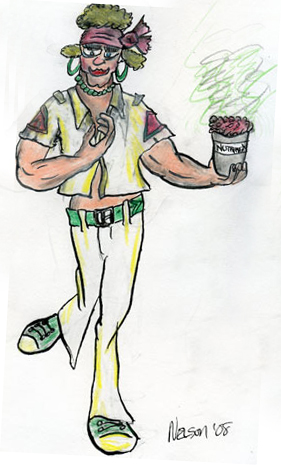
\includegraphics[height=60mm]{corps/chapitre3/img/simon.jpg}
\end{floatingfigure}

Être préposé au centre nutritionnel signifie qu’à raison de trois fois par jour, jamais plus et parfois moins, l’on s’occupe du Nutrisuz, une marque de commerce appartenant à la multinationale Monsanto. Il s’agit d’une nourriture industrielle très économique, une base alimentaire élaborée pour des bénéficiaires âgés, que l’on retrouve à la grandeur des provinces canadiennes et dans plusieurs états américains. Encore une fois, le Québec n’a rien inventé. La trouvaille est plutôt attribuable au docteur Anton Suzkinne, un chimiste d’origine russe faisant carrière chez Monsanto.

Le principe est simple. Tout ce qui est nécessaire pour la santé est présent dans cette purée. On dirait une sorte de gruau sans goût, mais riche en protéines, glucides et lipides, sans oublier un savantissime dosage de produits génétiquement modifiés, auquel on ajoute les suppléments individuels (sur ordonnance), ainsi que les arômes et colorants requis, tous tirés de substances artificielles. Le catalogue de Monsanto fait état de 750 saveurs chacune livrable en moins de 24 heures en contenants de cinq litres.

En cas de contre-indication, il existe du Nutrisuz Base, une nourriture insipide n’offrant que l’essentiel de l’essentiel, auquel (sur ordonnance) on rajoute mécaniquement ce que la personne doit et peut assimiler. Ainsi, le vieillard numéro BSL-34567-98 reçoit un plat de manger mou qui lui est propre, c.-à-d. qu’un voisin ne saurait avaler, un plat vitaminé où ont été incorporés tous les médicaments dont il a besoin. Idem pour les saveurs du matin, du midi ou du soir; la panoplie est assez vaste. Le logiciel choisit au hasard parmi celles qui ont été incluses dans la fiche du bénéficiaire, à sa demande. Cela constitue une petite surprise qui évite l’écœurement et les dépressions. Par exemple, le manger mou du matin sera aux fraises, celui du midi au poulet teriyaki et celui du soir, à la sole meunière. Le lendemain ce sera œufs, poutine cajun et dinde aux marrons. Et ainsi de suite. On a compris pourquoi les arômes et colorants ne pouvaient être d’origine naturelle.

Avec Chicot, un immigrant belge viscéralement homophobe qui le déteste pour le battre, Shimoune est présent cinq jours par semaine entre 8 h et 10 h le matin, entre midi et 14 h, puis entre 17 h et 18 h. En raison du fait que leur quart est divisé en trois blocs entrelardés de creux à rien faire, le CRG les paie quand même pour huit heures, même s’ils n’en font que six. Les vendredis après-midi, Ophélie Marcotte vient se joindre à eux. Préposée à temps partiel, elle assume en sa totalité le quart de fin de semaine. D’où sa présence du vendredi après-midi, question de s’assurer que tout baignera dans l’huile, puisqu’elle sera seule pendant les deux jours qui suivent.

Voilà un arrangement horaire qui laisse bien du temps à l’ignoble Chicot pour poser ses mines, des mines qu’arrive parfois à désamorcer Shimoune et à transférer à son avantage. Ainsi, il y a deux mois, le Belge avait dissimulé les poches de Paxil et de Zyban, des antidépresseurs lourdement utilisés en CRG, afin de rendre le quart d’Ophélie «inoubliable». Quand, à la fin de son premier service, à 10 h. le samedi matin, la jeune femme reçut du système un message selon lequel il n’y aurait pas assez de Paxil et de Zyban pour les préparations de Nutrisuz du midi, elle tenta de joindre Chicot, lequel se fit un malin plaisir de ne pas répondre. En panique, elle communiqua alors avec Saint-Pierre qui, flairant le coup fourré, accourut. Il fouilla dans tous les recoins du centre nutritionnel et finit par repérer les deux poches au fond d’un cagibi à désinfectant.

En clignant de l’œil à Ophélie, il referma l’armoire sans ne rien toucher et appela la sécurité.

- On n’a plus de Paxil et de Zyban pour la fin de semaine, déclara-t-il. Va falloir que j’aille en chercher dans l’entrepôt du sous-sol et moi, j’ai pas le code pour entrer là.

Ce qu’il fit, accompagné d’un agent de la Sécu, lequel, de retour à son bureau dût faire un rapport d’incident. C’est ce qui explique que le lundi matin, Amédée Chicot fut accusé de «négligence en matière d’approvisionnement» sans qu’il puisse se défendre. Eut-il essayé de le faire, il aurait eu l’air un peu idiot; il aurait suffi d’une demande à la Sécurité pour que la Direction puisse visionner la vidéo - car elle existait sûrement - de Chicot en train de fouiner dans le cagibi à désinfectant. Un blâme fut même ajouté à son dossier d’employé. Depuis ce jour, quoi que Shimoune dise, quoi qu’il fasse, la belle Ophélie le trouve génial ! Dommage qu’il soit affligé de mœurs aussi discutables !

Mais doit-on préciser que dans un centre nutritionnel, nul n’est besoin de technicien en cuisine ou en pharmacie ? Un préposé sans qualifications particulières suffit, ce qui est le cas de Shimoune qui n’a jamais terminé son cégep ou d’Ophélie qui s’est spécialisée en poésie innue à l’Université du Québec à Rimouski. C’est d’ailleurs une des raisons pour lesquelles Chicot les déteste tant. Lui, il a étudié des années pour devenir patron de cuisine. Il est passé par de nombreux restos, a servi, toque sur la tête, sous de nombreux chefs, tout cela pour aboutir à 41 ans, dans «le CN d’un CRG de merde», dans un «pays pourri» loin de Montréal, de New York, de Bruxelles. Lui qui se voyait maître queux aussi couru que craint, prépare aujourd’hui du manger mou, cette «putain de saloperie de Nutrisuz à la con», avec pour gâte-sauces, une «lopette» et une «meuf», deux «tarés complètement nuls» !

Car le travail y est désolant. Lorsqu’un bénéficiaire se présente à la cafétéria, salle aux effluves d’eau de javel, il commence par faire la queue au comptoir où l’accueille un assisté social bénévole qui lui capte son émetteur personnel (EP). Le segment pertinent de l’info dont regorge la puce, dispositif essentiel à toute vie, surtout quand on est vieux ou, pire, pensionnaire d’un CRG, est immédiatement traité par le système du CN. Si tout est en ordre, ce qui signifie que le petit vieux n’est pas censé être enfermé au sous-sol ou être décédé ou être grabataire, un timbre se fait entendre. Dès lors, Saint-Pierre ou Marcotte, mais jamais Chicot, place un contenant d’ABS d’un litre sous un périphérique d’ordinateur appelé «malaxeur sanitaire». C’est cette machine intelligente qui y injecte, comme les couleurs chez un quincaillier vendeur de peinture, la bonne dose de Coumadin, de Syntroïd, de Paxil, d’acétaminophène, etc. Le Viagra avait été retiré de la liste un an après le début des CRG, ce qui n’avait même pas soulevé de grogne dans les 2P. Selon les préférences qui apparaissent sur le fichier quantique du bénéficiaire, le Nutrisuz est chauffé ou servi froid. L’opération ne dure que cinq secondes.

Dès qu’il a fini de suçoter son manger mou, le vieux doit aller rincer son plat sous un des cinq robinets d’eau tiède prévus à cette fin. Cela lui permet, juste à côté, de l’emplir d’eau froide, de limonade ou de thé chaud; c’est à son goût. Pour Dart Vader, c’est un de ses moments favoris de la journée. Ciblant bien ses tables, il s’assoie sans attendre d’invitation et, avec une serviette de papier, entreprend de se récurer le «trou» respiratoire. L’impact de son humour est généralement immédiat.

Au fur et à mesure qu’ils ont fini de se sustenter, les vieux qui n’ont rien à discuter, surtout pas le bout de gras, quittent la cafeteria à petits pas mesurés. Mais avant, ils s’assurent qu’un bénévole les décharge de leur plat et de leur cuillère pour les déposer dans une grande laveuse électronique. Là, ces ustensiles sont aseptisés, prêts à servir de nouveau.

- Rappelons que tout le système repose sur les économies énormes que réalise l’État, une machine fabuleuse qui doit pouvoir digérer ses Boomers, avait expliqué récemment le gros Turcotte lui-même. Ainsi, avant la Loi 173, l’activité gouvernementale – je vous parle de l’ensemble des postes budgétaires afférents - qui consiste à s’occuper des personnes âgées coûtait jusqu’à 64 % de plus qu’aujourd’hui. Pour illustrer, on peut prendre l’exemple du CRG-BSL ici à Rimouski, où deux préposés et demi arrivent à sustenter, sans virer fous, plus de 840 bénéficiaires, de deux à trois fois par jour. Un miracle de gestion et de logistique !

Bien beau, mais dans son for intérieur, Timothée ne peut concevoir que l’on nourrisse les gens de cette façon. En ce sens, il est d’accord avec Ti-Dédé, c’est-à-dire Thierry-Ian Dennis-Dubeau (T.I.D.D), le charismatique leader des Verts et chef de l’opposition à Québec, qui, demain, est sensé venir visiter le Centre avec un cortège de journalistes. Évidemment, c’est une pensée qu’il garde bien pour lui; il ne la partage même pas avec Saint-Pierre, surtout qu’il ne le rencontre que dans l’établissement, enclave sinistre où les cafards électroniques sont omniprésents. Pire que dans ce roman de George Orwell dont il a oublié le nom.

On a compris qu’il n’était pas une personne aussi cultivée qu’il ne le souhaiterait. Avant d’être muté au CRG-BSL dans les mois qui suivirent la création de ces établissements, Timothée était agent de bureau senior, un classe IV, ce qui n’était pas rien, à la direction régionale du ministère de la Santé, où, attestation collégiale en poche, il était entré en 2015 à l’âge de 25 ans. Mais auparavant, il avait dû se farcir deux ans d’études en soins infirmiers pour plaire à sa mère; elle exigeait qu’il lui soit utile, «utile à ton tour», disait-elle en tapant du pied. Malheureusement pour elle, il avait dû abandonner cette formation cauchemardesque, étant incapable de supporter la vue du sang. Une petite hémorragie pouvait lui faire perdre tous ses moyens.

Il entend encore sa mère :

- C’est pas si terrible que ça, du sang ! C’est rien que la vie !

Aucune menace n’ayant pu régler sa phobie, il avait bifurqué vers la technique informatique et s’était décroché, sans passion aucune, un certificat en informatique d’affaires. D’où son statut d’agent classe IV. Avec un tel CV, les autorités du CRG-BSL n’avaient pas hésité à lui donner la responsabilité d’une section, la 5 Nord avec ses 56 vieillards, qui plus est, avec grade de CS-1. Quasiment une promotion ! Et même pas besoin d’avoir appris l’anglais !

Un léger frottement sur le cadre de porte de son bureau le tire de sa réflexion.

- Bonjour Madame Bellow, fait-il à l’ex-bibliothécaire avec la même révérence marquée que s’il s’adressait à un ancien allumeur de réverbères.

- Je m’excuse de vous importuner, Monsieur Tardif, mais je n’ai plus rien à lire, sourit-elle en lui présentant de ses deux petites mains ratatinées, quatre livres de poche. J’ai terminé le dernier hier soir.
Timothée s’empare des livres.

- Aimeriez-vous avoir d’autres Giono ? J’en ai trois ou quatre autres, si vous voulez.

- Oh ! Ça sera parfait, Monsieur Tardif. Jean Giono c’est très bien. Très bien même.

- Je vous amène ça demain, Mme Bellow. Mais faut pas le dire à personne, c’est promis ?

- Promis, monsieur Tardif.

Et le fantôme des temps d’autrefois repart dans le silence de ses pantoufles roses.

Ce côté «contrebandier pas méchant» de Timothée ne l’empêchait pas de diriger, depuis cinq ans, une petite équipe de préposés aux bénéficiaires. Ainsi, de 8 h à 16 h, son quart de travail à lui, deux gaillards l’assistaient. Il pouvait s’agir de Steve Grenier ou de son comparse Laurent Bérubé, deux émetteurs de farces idiotes et vulgaires, ou encore de Ronnie Ross - ça se prononce «Wrâné Wrâss» - ou de son complice des coups sournois, Charles Chuck Chicoine - faut dire «Tchok Tchicouaine» - ou encore, d’un petit nouveau appelé Mérovée d’Anjou. Ils étaient donc trois employés, ce qui était amplement suffisant pour s’occuper de sept salles pleines de vieux, dont certains dégoulinant par toute sorte de bouts.

De 16 h à minuit, deux PB venaient prendre leur relève. Personne voulant être de ce quart, Timothée devait produire la liste des affectations au moins un trimestre d’avance. Et même là, certains se vengeaient. Ainsi, ces couches dégoûtantes dans le tiroir principal du bureau de Timothée, ce vieillard oublié trois heures durant sur une cuvette, ce poivre en poudre ajouté au manger mou de grabataires, etc. Enfin, de minuit à 8 h, il fallait se fier au personnel de nuit, des PB comptés sur les doigts de la main qui relevaient de la directrice des soins infirmiers sans avoir de comptes à rendre à Timothée, ce qui convenait parfaitement à ce dernier. Est-on obligé, dans la vie, de multiplier les sources de problèmes ?

À ces gens s’ajoutaient, au jour le jour, des assistés sociaux qui venaient «donner des heures» pour pouvoir manger ou se faire soigner et à qui on confiait exclusivement les tâches dites ingrates : changer les couches dans les salles 3P et SP (aucune couche n’est tolérée dans les 2P; advenant qu’il faille en arriver là, la bénéficiaire est mutée en 3P…), donner le manger mou aux vieillards impotents en 3P et, parfois, en SP, servir le manger mou à la cafeteria, piloter les zambo (sorte de balayeuse, laveuse et cireuse combo) dans les passages et les salles, tondre la pelouse, pelleter la neige, jouer de la musique dans les salons communautaires, pièces réservées aux résidents en 2P et, sur approbation expresse, aux nouveaux en 3P, etc. Et si jamais on manquait d’assistés sociaux, on mobilisait les pensionnaires des salles 2P, cela à leur grande indignation. En cas de force majeure, on avait recours aux bénéficiaires les moins poqués du Centre régional de réadaptation et d’hébergement pour handicapés intellectuels sis deux coins de rue plus loin.

Par sa porte grande ouverte, Timothée perçoit des imprécations en provenance du poste de garde situé à quelques enjambées de son bureau. C’est Laurent Bérubé qui, d’après ce que le CS-1 voit après s’être étiré le cou, est en train de fouiller sans ménagement le bonhomme Martel, un résidant bien malgré lui qui accepte mal sa nouvelle vie de «bénéficiaire». Surtout que son épouse des 51 dernières années est elle-même pensionnaire dans une salle 2P sur le même étage.

- Vous l’avez caché où, votre bouteille, le pére ?

- J’en n’ai pas de bouteille, maudit voyou !

- Vous sentez la tonne à plein nez, vieux menteur !

- M’a t’en faire des «vieux menteurs», espèce de mal élevé. J’vais porter plainte.
Pour ne pas que la scène ne dégénère davantage, Timothée manœuvre sa Saguewanish vers le poste de garde.

- Laisse tomber, Laurent, je m’en occupe.

- Visiblement, le gaillard n’apprécie pas.

- C’est comme tu veux, le Motté. C’est toi le chef !

Et il recule se réfugier de l’autre côté du comptoir, le front plissé de rides malicieuses.

- Venez, Monsieur Martel, on va aller se calmer, fait le chef de section en marchant à côté de sa bécane.

C’est comme s’il avait appuyé sur un bouton, clic ! À coups de paroles courtes et saccadées, le petit vieux se met à déverser l’excédent de son exaspération accumulée. Il en ressort que le CRG-BSL n’est pas une maison de repos pour vieux, mais un abattoir où l’État a embauché des fier-à-bras sans classe, des brutes, des moins que rien, des sans cœur qui séparent les conjoints, qui défont les familles, qui maltraitent les gens, des gens qui ont trimé dur toute leur vie, qui ont payé des impôts comme des idiots pendant une soixantaine d’années, pour finir ravalés au rang de bêtes, des bêtes sans droit «juste bonnes pour attendre la mort».

- Jamais, on ne m’a manqué autant de respect dans ma vie !

Timothée aide le vieillard à s’asseoir sur son lit.

- Monsieur Martel, faites seulement un peu plus attention. La bouteille de rhum que vous cachez dans la poche de linge sale de votre garde-robe, il y a trop de monde qui vous voient vous en servir. Soyez juste un peu plus discret.

- J’en peux plus !

- Si Bérubé fait un rapport, je vais être obligé de donner suite. Vous connaissez la procédure, va falloir vous amener chez les Papyblues. Mais là, faites-vous-en pas, je vais aller arranger ça.

Atterré, le vieil homme reste coi. Timothée a utilisé le mot magique, Papyblues, l’horrible patronyme des tourmenteurs psychopathes qui rôdent dans les dédales du sous-sol.

Hélas ! deux lits plus loin, l’Illuminé démarre son cirque habituel.

- «Malheur à ceux qui de bon matin courent après les boissons enivrantes et qui bien avant dans la nuit sont échauffés par le vin !» C’est écrit dans la Bible, misérables impies ! Et même Saint Luc le dit dans son Évangile : «Car il sera grand devant le Seigneur. Il ne boira ni vin, ni liqueur enivrante, et il sera rempli de l’Esprit Saint dès le sein de sa mère !» Pourquoi ne craignez-vous pas la colère de Dieu ? Vous êtes en train de transformer ce lieu de méditation et de préparation vers la vie éternelle en filiale sordide de Sodome et Gomorrhe !

- Monsieur Savoie, calmez-vous, dit-il à l’illuminé. Monsieur Martel a besoin de se reposer.

Jean-Roch Savoie, un authentique Bleuet d’Alma, s’était établi dans le 3e Rang de Saint-Fabien (25 kilomètres de Rimouski) vers la fin des années 2010. Là, il avait démarré une sorte de secte néo-catholique qui lui avait permis de ne pas trop travailler pendant une vingtaine d’années. Relativement inoffensif, il embêtait néanmoins les autres pensionnaires du 5e Nord avec ses visions apocalyptiques et ses certitudes d’être de plus en plus près d’un Dieu terriblement courroucé par rapport à sa Création.

- Tais-toi donc, espèce de fanatique !

Martel semble pour le moins très agacé.

- Chef, ajoute-t-il, je vais te dire quelque chose, service pour service.

- Vous ne me devez rien, Monsieur Martel.

- Moi, mon ‘tit garçon, je n’ai jamais eu de dettes de toute ma vie ! Écoute-moi bien, j’vas t’le dire juste une fois. Ton Saguewanish a été saboté. Là il fait du bruit, mais fais bien attention, il est à veille de sauter. À ta place, je ne le monterais plus.

- Comment vous savez ça ?

- Je les ai vus faire vendredi passé quand tu es allé jaser dans le bureau d’Alcide. Tu avais laissé ta bécane dans le passage, fait qu’ils en ont profité.

- Qui ça ?

- Il est écrit: «N’abandonne pas un vieil ami, le nouveau ne le vaudra pas !» coupe l’Illuminé. Réfléchis Martel, réfléchis avant de vendre tes frères à Pharaon ! Car il est aussi écrit: «Comme tu as fait il te sera fait : tes actes te retomberont sur la tête».

- Étouffe, vieux sans dessein !

Puis, regardant Timothée:

- Je peux pas de dire ça, chef, tout ce que je peux te dire c’est d’amener ton saguigui au garage.
Au même moment, Timothée voit filer devant la porte de la salle l’ombre furtive de Robespierre Alcide.

- Parlant du loup, fait observer Martel.

Robespierre arrive probablement des commodités. D’où pourrait-il venir pendant les heures d’ouvrage, sinon de là ? Et où pourrait-il aller, sinon là ? Comme on ne le remarque jamais au salon des employés, qu’il mange dans son bureau, qu’il ne fait partie d’aucuns comité et qu’il ne fréquente jamais les fêtes ou les partys, personne ne s’entretient avec lui, sauf Timothée, ravi d’avoir trouvé quelqu’un lui ressemblant quelque peu, façon de parler. Tant et si bien que le personnage est devenu un ami comme l’est Shimoune Saint-Pierre, quelqu’un avec qui il peut échanger.

Inquiété par les propos du père Martel, le CS-1 quitte la salle sans prendre place sur son Saguewanish et, de son petit pas poussif, se dirige vers le bureau de Robespierre, traînant sa trottinette derrière lui.

\begin{floatingfigure}[r]{35mm}
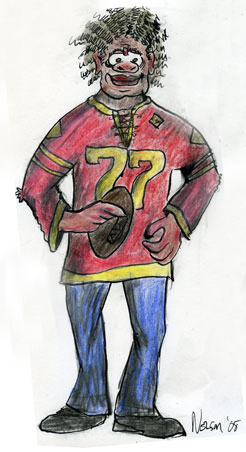
\includegraphics[height=60mm]{corps/chapitre3/img/alcide.jpg}
\end{floatingfigure}

Le grand-père Alcide, un footballeur haïtien (un joueur de soccer, pas de football américain), avait immigré au Québec il y a bien longtemps et, depuis, la famille s’était signalée en sport et en loisirs. Lui, Robespierre, il était directeur des loisirs du CRG-BSL. Fier détenteur d’une maîtrise en éducation physique et d’un bac en récréologie gérontologique de l’Université Laval, il en avait même porté les couleurs au football interuniversitaire. Pourtant, son actuelle fonction avait un sérieux inconvénient pour quelqu’un d’aussi qualifié que lui; au cours des quatre dernières années, on ne lui avait pas consenti de budget. Zéro ! Même pas de quoi acheter deux raquettes de badminton au Dollorama. Les vieux des dortoirs 2P en était réduits à traîner leurs savates dans les salles communautaires, à parler du bon vieux temps, à jouer aux cartes, à regarder la télé, à sommeiller ou, plus rarement, à s’amuser avec le terminal du quanticordi. Le gymnase avait été converti en salon du personnel avec certaines facilités alimentaires et récréatives. Quant à la piscine, on l’avait tout simplement vidée et condamnée.

Puisque le poste de directeur des loisirs est considéré obligatoire dans la Loi constituante des CRG, Robespierre faisait partie des effectifs de celui du Bas-Saint-Laurent et, à ce titre, était tenu d’être présent cinq jours semaine. Le pauvre diable passait ainsi ses grandes journées enfermé dans son bureau, un réduit situé, à la limite des ailes nord et centre du 5e étage, à proximité de l’officine de Timothée. Qu’y faisait-il ? Personne, à part ce dernier, ne savait qu’il y lisait des romans et surtout des ouvrages psychologiques, un dada qu’il cultivait avec délectation, qu’il écrivait de la poésie, qu’il faisait des redressements et poussait des pompes, enfin, qu’il entretenait un monde virtuel où une communauté essentiellement québéco-haïtienne venait revivre les aventures de Toussaint Louverture telles que réécrites et lourdement musclées par Robespierre.

- Tu sais Timothée, lui avait-il raconté un jour, le père de mon grand-père, Terrence-Raoul Alcide, qui était un peu chimiste ou, plutôt, alchimiste autodidacte, avait trouvé une façon de mélanger des herbes, de la levure, de l’eau avec d’autres trucs ignobles. Il faisait chauffer et mijoter cette soupe pendant presque deux jours, laissait décanter et remplissait de petits flacons qu’il vendait dans tous les bars des Gonaïves. Il avait appelé son épouvantable mixture «Pétépano». Il suffisait d’en boire quelques gorgées pour devenir, peu après, en virile situation de fournir, à leur satisfaction, autant de dames que la bienséance communale pouvait l’exiger. D’où le nom «Pétépano». C’est cette trouvaille qui permit à Terrence-Raoul de bien nourrir sa famille et faire en sorte que son aîné devienne un footballeur étoile.

Si Robespierre s’était complu dans une anecdote aussi savoureuse, c’était pour illustrer que chez les Alcide, aussi bien en Haïti qu’au Québec, il y avait une tradition d’entraide. Il fut un temps où toutes les semaines, son grand-père, joueur de soccer, allait porter des caisses de bananes plantains dans un centre communautaire de Montréal-Nord, de la nourriture qu’il avait payée de sa poche. Son propre père, lui-même ailier droit au soccer, mais surtout rappeur et slameur, se produisait gratuitement partout où il estimait pouvoir rendre service à la communauté. Et lui ?

Il n’avait pas répondu. Mais à petits coups de déductions, de mini observations, d’inavouables spéculations et de fines intuitions, Timothée avait fini par l’associer, à tort ou à raison, à la fourniture de pilules du bonheur, un service des temps modernes que Robespierre pouvait rendre à la communauté du CRG.

- Qu’est-ce que je peux faire pour toi, mon ami ?

Le tristounet binoclard s’assied sur la seule chaise à ne pas être encombrée de livres. Pendant cinq minutes, il va tourner autour du pot sans rien oser. Puis, sans transition :

- Tu as sûrement une idée sur ces fameuses pilules qui n’existent pas ?

- Ouais, les pilules du bonheur.

Timothée vise l’ahurissant capharnaüm, plus particulièrement cette masse murale hétéroclite constituée de livres empilés et de souvenirs du Rouge et Or, l’équipe de l’Université Laval.

- J’en cherche. Euh, si jamais tu entends parler de quelque chose …

Il se lève, les yeux sur le souk ambiant, et gagne le corridor sans que Robespierre lui réponde.

Son attention est immédiatement portée vers Luce Morency, une ancienne jolie fille maintenant âgée de 86 ans. Elle s’est encore évadée de son lit de la salle 3P-L 6 Nord, laquelle, heureusement, n’est pas de la juridiction de Timothée. La bonne femme n’a pas ses dents, ses cheveux sont longs, laids, sales et en désordre. Comme elle est nue, sa maigreur pendouillante donne la chair de poule aux gens qu’elle croise. Timothée se pince la boucle d’oreille et dit :

- 6e Nord, code magenta !

On lui répond et il rapporte la fugueuse. Dans l’attente qu’on vienne la chercher, il lui prend néanmoins la main, «venez avec moi, madame Morency», et la fait s’asseoir sur une des chaises près de l’ascenseur. Il en fait autant sur le siège voisin et lui parle du lac Saint-Mathieu où la vieille dame habitait un chalet converti en maison. Pendant une trentaine d’années, elle y avait exploité une petite affaire de location de roulottes rapaillées qu’elle destinait aux villégiateurs venus de la ville. Puis un jour, un de ses amants était disparu avec la caisse, juste avant un dépôt, et moralement abattue, aux prises avec des dettes insolvables, Luce Morency avait fait faillite. Le reste n’avait été que débâcle, désastre et misère noire.

Peu après, un préposé du 6e se pointe, c’est le gros Lavoie, un calamiteux qui mange à tous les râteliers. Tellement qu’il possède trois immeubles d’habitation au Centre-ville de Rimouski. Il a amené un fauteuil roulant et une couverture dans laquelle il drape la mère Morency. En la morigénant comme une pouilleuse, il la roule jusque dans l’ascenseur et ils disparaissent. Quel fils de salaud !

- Je l’ai connue, dans le temps, la Luce Morency !

La mère Thériault qui décidément ne pouvait rater une si belle occasion, brandit son sourire malicieux des grands jours.

- C’est d’valeur qu’elle vieillit aussi mal ! Méchante belle femme, dans le temps ! Dans le temps de nos bals à l’huile du lac Saint-Mathieu. Elle était tout le temps là. Mais on aurait dit qu’elle se méfiait de moi … Pourtant !

Sans plus tenir compte de la radoteuse, Timothée file vers son bureau, question de vérifier si rien qui ne peut attendre s’est affiché, de signaler sa fin de quart au système et de placer son terminal en mode veille.

Quand la cage de l’ascenseur s’arrête au 5e, Marie-Odile Tremblay, une forte femme de 37 ans que l’on surnomme la Bitch, s’y trouve déjà et semble sérieusement occupée à contempler le tableau indicateur. C’est une agente de sécurité sans charme, ni grâce, ni coquetterie, une personne dont on craint la colère, qu’on n’a jamais vue sourire et qu’on croit délatrice active. N’est-elle pas cette flic maison qui a récemment mis au jour un racket de nourriture clandestine, essentiellement du raisin sec, des abricots séchés et des noix, que deux préposés du 4e Centre, des misérables désormais sans emploi, revendaient à des détenteurs de monnaie à plume ?

Timothée n’ose la saluer, même si, depuis quelque temps, il la soupçonne d’être à l’origine de l’avatar avec lequel le sien s’amuse holographiquement depuis une semaine ou deux. La femme tourne légèrement la tête, comme pour le regarder. On dirait qu’elle nourrit les mêmes soupçons.

Mais au moment où les portes se referment, une main brune tout en muscles se glisse à l’intérieur, ce qui enclenche automatiquement la réouverture.

- Je m’excuse, fait Robespierre Alcide. Il est 16 heures et …

Habitué à ce que personne ne s’intéresse à lui, il ne termine pas sa phrase.

Arrivés au 2e, le CS-1 et l’agente de sécurité sortent. Elle parce que c’était SA destination, la Sécurité occupant toute l’aile sud du 2e, lui parce qu’il se croyait rendu au rez-de-chaussée.

- Au revoir, Marie-Odile, déclame Robespierre, un sourire tout craquelé sur le bord des lèvres.

Sans lui retourner sa politesse - une politesse intéressée ? - elle le regarde avec sévérité. Et c’est avec le même air qu’elle fixe cet autre «perdant» qui tente bêtement de s’excuser. Excédée, elle hausse les épaules et file sur son Saguewanish, toutes voiles déployées. Un Saguewanish qui ne fait pas de bruit. Humilié encore une fois, Timothée entreprend de pitonner la console murale de l’ascenseur. Pourquoi Robespierre ne l’a-t-il pas attendu ? À cause de sa requête de tout à l’heure ?

Mais tout près, dans une officine à peine plus grande que la sienne, un sexagénaire à bouc, selon cette mode grotesque qui frappa l’Occident dans les années 2005-2010, lui fait signe de la main avec insistance. Timothée hésite et se pointe le thorax de l’index en hochant de la tête à répétition. L’autre fait signe que oui en répétant son geste. Le CS-1 embraye donc sa vieille bécane. Il sait que cet étrange personnage qu’on ne voit jamais nulle part, lui non plus, est Sébastien Larose, le dernier syndiqué de la Fonction publique du Québec. Tous les autres sont soit décédés, soit retraités, soit devenus cadres.

La formule Rand ayant été déclarée inconstitutionnelle par la Cour Suprême en 2018, Québec l’avait supprimée l’année suivante pour s’éviter un très juteux recours collectif. En conséquence, plus personne parmi les nouveaux employés de l’État n’avait voulu adhérer au syndicat. Le vieux Sébastien était désormais le seul de son espèce. Ce qui signifie qu’en vertu des lois du Travail en vigueur, le syndicat devrait être dissolu par le Lieutenant-gouverneur en conseil le jour où Larose partirait. En attendant, il cumulait les postes de président, de secrétaire, de trésorier et agissait comme assemblée générale. Ne sachant trop quoi en faire, voulant s’éviter une structure patronale syndicale, les autorités du CRG-BSL avaient préféré placer cet énergumène d’un autre âge dans un bureau confortable où on lui foutait la paix dans l’attente de sa retraite, ce qui devrait arriver dans les huit prochains mois. Croyait-on en haut lieu !

- Excuse-moi, mon homme, fait-il un crayon à la main, je cherche un mot de dix lettres, dix lettres, qui signifie «rationalisation administrative efficace» et qui commence par les lettres HO …

Il a prononcé «mon homme» comme seuls les Bas-laurentiens savent le faire. Vouloir respecter le son, il faudrait écrire «mânem».

- Euh ! Dix lettres ?

- Ouin, p’is ça finit par un E…

- Euh ! Rationalisation administrative efficace, attendez …

- Dix lettres.

- Je l’ai. C’est HOLOCAUSTE.

- Ahhh ! Génial ! Merci mon homme !

Timothée ressort du petit bureau et reprend place sur son Saguewanish. Il s’engouffre dans l’ascenseur et le quitte un étage plus bas, en face du portrait couleur de Sylvain Turcotte, l’homme fort du régime libéral. Ignorant quelques quolibets d’usage, il sort de l’édifice et roule jusqu’au stationnement où il aperçoit Shimoune Saint-Pierre presque nu, couché sur le devant de son automobile électrique en train de prendre le soleil de l’après-midi.

- Beau temps pour s’étendre ! T’as fini ta journée, Momo ?

- Ouin.

- Saint-Pierre ajuste ses verres fumés.

- C’est pas de mes affaires, mais je viens de voir le gros Lavoie placer un bout de papier dans ton pare-brise.
- Ah !
Timothée salue son ami et se dirige vers la section du stationnement - c’est la plus éloignée –qui est réservée aux voitures à essence. Effectivement, quelque chose de flageolant a été glissé sous les essuie-glaces de sa bagnole, concentré de rouille construit en 2013. C’est une feuille toute dégueulasse, on la dirait souillée de matières abominables, où on le traite de «gros motté téteux de boss qui, un jour, va se faire casser sa yeule de rat». Sans colère, il chiffonne le brouillon et va le jeter dans un bac à recup trois pas plus loin.

Pourquoi le persécute-t-on tant ? Pourquoi le déteste-t-on tant ? Il n’en est pas certain. Possiblement parce qu’il ne parle à personne, parce qu’il est chef de section, classe 1, parce qu’il ne fréquente pas le club social, à l’instar de Robespierre, de Shimoune ou du vieux Sébastien Larose. Sûrement parce qu’il a une tronche louche avec ses barniques épaisses, ses cheveux trop éclaircis, sa trottinette qui en arrache, sa chemise tachée de sauce à spaghetti, sa dégaine de perdant. Toute cette méchanceté gratuite, cette bête incompréhension, est, la plupart du temps, lourde à porter et, comme c’est le cas présentement, l’emplissent d’un cafard qui l’habitera encore, il le sait, bien après qu’il sera rendu chez lui. Aimerait-il pouvoir se venger, ruer, hurler, frapper, impressionner, susciter le respect, obtenir du gros Lavoie qu’il lui demande pardon ? Peut-être, mais ce n’est pas vraiment dans sa nature.

Sans dire un mot, il place le bruyant Saguewanish dans la malle de la bagnole, quitte le terrain du CRG et prend la direction de Nazareth. En cette fin d’après-midi de juillet, l’air du fleuve rend possible, voire délectable, la chaleur extraordinaire - à Montréal, ils disent «accablante» - qui assaille l’Est-du-Québec depuis quelque temps. Les gens sont partout sur les trottoirs, les balcons, dans les parcs, sur la promenade du Fleuve, sur les pistes cyclables, sur les terrasses. On rit, on sourit, on crie, on s’arrose, on s’attrape, on s’aime, on est heureux. Mais lui, Timothée, il roule plutôt vers autre chose, vers une sorte de tombeau sombre, sale et hostile où l’humidité sera étouffante et, comme c’est de plus en plus le cas, nauséabonde.

- Merde, j’ai oublié les sacs de la mère Loubert !
